\documentclass[aspectratio=169,10pt]{beamer}

\usepackage{array}
\usepackage{booktabs}
\usepackage{graphicx}
\usepackage{amsmath}
\usepackage{amssymb}
\usepackage{tikz}
\usetikzlibrary{arrows.meta,calc,positioning,shapes.geometric,fit}
\newcolumntype{L}[1]{>{\raggedright\arraybackslash}p{#1}}

% DGIST ISL Custom Color Palette
\definecolor{islteal}{RGB}{43,133,147}
\definecolor{islred}{RGB}{203,76,65}
\definecolor{isldark}{RGB}{52,61,67}
\definecolor{islnavy}{RGB}{31,55,95}
\definecolor{islmuted}{RGB}{92,101,108}
\definecolor{isllight}{RGB}{236,241,243}
\definecolor{islgold}{RGB}{184,119,20}
\definecolor{islgreen}{RGB}{44,145,91}
\definecolor{islpurple}{RGB}{130,58,160}

\newcommand{\deckdate}{2026.08.21}
\newcommand{\labname}{DGIST Intelligent Systems and Learning Laboratory}

\setbeamersize{text margin left=0.65cm,text margin right=0.65cm}
\setbeamertemplate{navigation symbols}{}
\setbeamertemplate{blocks}[rounded][shadow=false]
\setbeamercolor{normal text}{fg=isldark,bg=white}
\setbeamercolor{frametitle}{fg=isldark,bg=white}
\setbeamercolor{footer}{fg=white,bg=isldark}
\setbeamerfont{frametitle}{series=\bfseries,size=\Large}
\setbeamerfont{normal text}{size=\small}

\setbeamertemplate{frametitle}{%
  \nointerlineskip%
  \begin{beamercolorbox}[wd=\paperwidth,ht=1.35cm,dp=0cm]{frametitle}
    \vskip0.45cm%
    \hspace*{0.74cm}\insertframetitle\par%
    \vskip0.05cm%
    \hspace*{0.74cm}{\color{islteal}\rule{0.68\paperwidth}{4pt}}%
    {\color{islred}\rule{0.20\paperwidth}{4pt}}%
  \end{beamercolorbox}%
}

\setbeamertemplate{footline}{%
  \leavevmode%
  \begin{beamercolorbox}[wd=\paperwidth,ht=0.34cm,dp=0.11cm]{footer}
    \hspace*{0.65cm}{\scriptsize\deckdate}%
    \hfill{\scriptsize Reinforcement Learning \& Robotics Track \quad $\vert$ \quad Week 03: Bellman Error \& DQN}\hfill%
    {\scriptsize\insertframenumber\,/\,\inserttotalframenumber}\hspace*{0.65cm}%
  \end{beamercolorbox}%
}

\newcommand{\bottomrulebar}{%
  \begin{tikzpicture}[remember picture,overlay]
    \fill[islteal] (current page.south west) rectangle ++(0.43\paperwidth,0.11cm);
    \fill[isldark] ([xshift=0.43\paperwidth]current page.south west)
      rectangle ++(0.34\paperwidth,0.11cm);
    \fill[islred] ([xshift=0.77\paperwidth]current page.south west)
      rectangle ++(0.23\paperwidth,0.11cm);
  \end{tikzpicture}%
}

\newcommand{\sectionlabel}[1]{%
  {\small\bfseries\color{islteal}#1}\par\vspace{0.14cm}%
}

\begin{document}

% ==========================================
% SLIDE 1: Title Slide
% ==========================================
\begin{frame}[plain,noframenumbering]
  \bottomrulebar
  \vspace{1.00cm}
  {\centering
    {\fontsize{22}{26}\selectfont\bfseries\color{islnavy}
      Week 03: Bellman Error and Deep Q-Networks\par}
    \vspace{0.22cm}
    {\fontsize{15}{18}\selectfont\color{islteal}
      Replacing Tabular Lookups with Parametric Function Approximators\par}
    \vspace{0.50cm}
    {\large\bfseries Reinforcement Learning \& Robot Learning Core Curriculum\par}
    \vspace{0.20cm}
    {\small Presented by \textbf{DGIST ISL Team}\par}
    \vspace{0.12cm}
    {\small\color{islmuted} \labname\par}
    \vspace{0.10cm}
    {\small \deckdate\par}
    \vspace{0.45cm}
    {\scriptsize\color{islmuted}
      Core Concepts: Bootstrapped Bellman Loss $\cdot$ Target Networks $\cdot$ Experience Replay $\cdot$ Diagnostic Baselines\par}
  }
\end{frame}

% ==========================================
% SLIDE 2: Paradigm Shift (Tabular -> Function)
% ==========================================
\begin{frame}{The Scaling Wall: Tabular to Function Approximation}
  \sectionlabel{Continuous and high-dimensional states require generalizable parameterization}

  {\centering
    \begin{tikzpicture}[
      box/.style={rounded corners=4pt, text width=6.5cm, minimum height=3.1cm, inner sep=6pt, font=\scriptsize, line width=0.9pt, align=left}
    ]
      % Left Card: Tabular
      \node[box, draw=islmuted, fill=isllight!60] at (3.5, 1.8) {
        {\bfseries\color{isldark}\normalsize Tabular Q-Learning (Week 02)}\\[3pt]
        \textbf{Lookup Table:} $Q[s, a] \in \mathbb{R}^{|S| \times |A|}$\\[2pt]
        $\bullet$ Updates affect \textbf{strictly one cell} $(s, a)$ at a time.\\[1pt]
        $\bullet$ Zero generalization across similar states ($s=1.01$ vs $s=1.02$).\\[1pt]
        $\bullet$ \textbf{Curse of Dimensionality:} Continuous robot states make tables impossible.
        \vskip3pt
        \centering
        \begin{tikzpicture}[scale=0.60]
          \draw[step=0.6, islmuted, thin] (0,0) grid (3.0,1.2);
          \node at (1.5, 0.6) {\tiny $Q[s, a]$ table};
          \draw[-{Latex}, thick, islred] (0.9, 0.3) -- ++(0.8,0);
        \end{tikzpicture}
      };

      % Right Card: Function Approximator
      \node[box, draw=islteal, fill=islteal!6] at (10.7, 1.8) {
        {\bfseries\color{islteal}\normalsize Parametric Q-Approximation (Week 03)}\\[3pt]
        \textbf{Model Prediction:} $Q_\theta(s, a) \approx Q^*(s, a)$ with weights $\theta$\\[2pt]
        $\bullet$ An update to $\theta$ \textbf{generalizes across state regions}.\\[1pt]
        $\bullet$ Scales to continuous observations, embeddings, and raw images.\\[1pt]
        $\bullet$ \textbf{Tradeoff:} Changing $\theta$ shifts values for \textit{many} states simultaneously.
        \vskip3pt
        \centering
        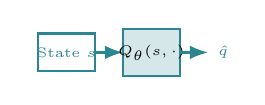
\begin{tikzpicture}[scale=0.60]
          \draw[thick, islteal, fill=white] (0,0.2) rectangle (1.2,1.0) node[pos=.5]{\tiny State $s$};
          \draw[-{Latex}, thick, islteal] (1.2,0.6) -- (1.8,0.6);
          \draw[thick, fill=islteal!20, draw=islteal] (1.8,0.1) rectangle (3.0,1.1) node[pos=.5]{\tiny $Q_\theta(s, \cdot)$};
          \draw[-{Latex}, thick, islteal] (3.0,0.6) -- (3.6,0.6) node[right]{\tiny $\hat{q}$};
        \end{tikzpicture}
      };
    \end{tikzpicture}
  \par}
\end{frame}

% ==========================================
% SLIDE 3: Visual Method Pipeline - Bellman Error to Loss
% ==========================================
\begin{frame}{Method Architecture: Constructing the Bellman Loss}
  \sectionlabel{Temporal-Difference (TD) learning transforms dynamic programming into supervised regression}

  {\centering
    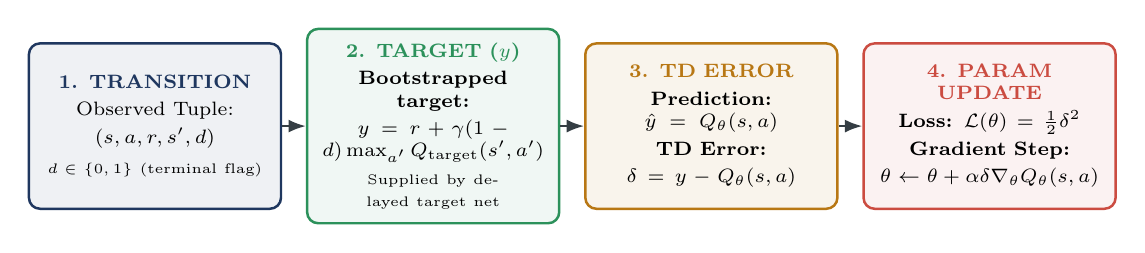
\begin{tikzpicture}[
      node distance=0.30cm,
      stage/.style={rounded corners=4pt, text width=2.85cm, minimum height=2.1cm, align=center, inner sep=5pt, font=\scriptsize, line width=0.9pt},
      arr/.style={-{Latex[length=2.2mm]}, thick, color=isldark}
    ]
      % 1. Transition
      \node[stage, draw=islnavy, fill=islnavy!7] (trans) {
        {\bfseries\color{islnavy} 1. TRANSITION}\\[2pt]
        Observed Tuple:\\[2pt]
        $(s, a, r, s', d)$\\[3pt]
        \tiny $d \in \{0, 1\}$ (terminal flag)
      };

      % 2. Bellman Target
      \node[stage, draw=islgreen, fill=islgreen!7, right=of trans] (target) {
        {\bfseries\color{islgreen} 2. TARGET ($y$)}\\[2pt]
        \textbf{Bootstrapped target:}\\[2pt]
        $y = r + \gamma(1-d)\max_{a'} Q_{\text{target}}(s', a')$\\[2pt]
        \tiny Supplied by delayed target net
      };

      % 3. Prediction & Error
      \node[stage, draw=islgold, fill=islgold!8, right=of target] (pred) {
        {\bfseries\color{islgold} 3. TD ERROR}\\[2pt]
        \textbf{Prediction:} $\hat{y} = Q_\theta(s, a)$\\[2pt]
        \textbf{TD Error:}\\[2pt]
        $\delta = y - Q_\theta(s, a)$
      };

      % 4. Loss & Gradient
      \node[stage, draw=islred, fill=islred!7, right=of pred] (loss) {
        {\bfseries\color{islred} 4. PARAM UPDATE}\\[2pt]
        \textbf{Loss:} $\mathcal{L}(\theta) = \tfrac{1}{2}\delta^2$\\[2pt]
        \textbf{Gradient Step:}\\[2pt]
        $\theta \leftarrow \theta + \alpha \delta \nabla_\theta Q_\theta(s, a)$
      };

      \draw[arr] (trans) -- (target);
      \draw[arr] (target) -- (pred);
      \draw[arr] (pred) -- (loss);
    \end{tikzpicture}
  \par}

  \vspace{0.14cm}
  \begin{columns}[T,onlytextwidth]
    \column{0.48\textwidth}
      \begin{block}{\small\color{islteal}\textbf{Non-Terminal Case ($d=0$)}}
        \footnotesize Target $y = r + \gamma \max_{a'} Q_{\text{target}}(s', a')$. Future values are discounted and bootstrapped from next state.
      \end{block}
    \column{0.48\textwidth}
      \begin{block}{\small\color{islred}\textbf{Terminal Case ($d=1$)}}
        \footnotesize Target $y = r$. At goal/failure termination, future return is strictly zero. Never bootstrap across true episode boundaries!
      \end{block}
  \end{columns}
\end{frame}

% ==========================================
% SLIDE 4: Concrete Numerical Walkthrough in LineWorld
% ==========================================
\begin{frame}{Concrete Walkthrough: LineWorld Arithmetic}
  \sectionlabel{Hand-traceable example: how the Bellman error translates into exact numerical loss}

  {\centering
    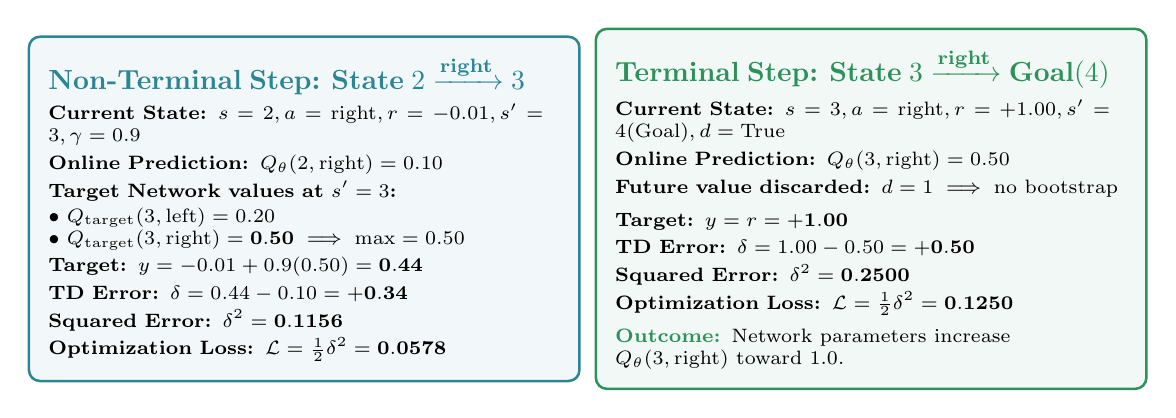
\begin{tikzpicture}[
      card/.style={rounded corners=4pt, text width=6.5cm, minimum height=3.3cm, align=left, inner sep=7pt, font=\scriptsize, line width=0.9pt}
    ]
      % Non-terminal step
      \node[card, draw=islteal, fill=islteal!6] at (3.5, 1.7) {
        {\bfseries\color{islteal}\normalsize Non-Terminal Step: State $2 \xrightarrow{\text{right}} 3$}\\[3pt]
        \textbf{Current State:} $s=2, a=\text{right}, r=-0.01, s'=3, \gamma=0.9$\\[2pt]
        \textbf{Online Prediction:} $Q_\theta(2, \text{right}) = 0.10$\\[2pt]
        \textbf{Target Network values at $s'=3$:}\\[1pt]
        $\bullet$ $Q_{\text{target}}(3, \text{left}) = 0.20$\\
        $\bullet$ $Q_{\text{target}}(3, \text{right}) = \mathbf{0.50} \implies \max = 0.50$\\[2pt]
        \textbf{Target:} $y = -0.01 + 0.9(0.50) = \mathbf{0.44}$\\[2pt]
        \textbf{TD Error:} $\delta = 0.44 - 0.10 = \mathbf{+0.34}$\\[2pt]
        \textbf{Squared Error:} $\delta^2 = \mathbf{0.1156}$\\[2pt]
        \textbf{Optimization Loss:} $\mathcal{L}=\tfrac{1}{2}\delta^2=\mathbf{0.0578}$
      };

      % Terminal step
      \node[card, draw=islgreen, fill=islgreen!6] at (10.7, 1.7) {
        {\bfseries\color{islgreen}\normalsize Terminal Step: State $3 \xrightarrow{\text{right}} \text{Goal}(4)$}\\[3pt]
        \textbf{Current State:} $s=3, a=\text{right}, r=+1.00, s'=4 (\text{Goal}), d=\text{True}$\\[2pt]
        \textbf{Online Prediction:} $Q_\theta(3, \text{right}) = 0.50$\\[2pt]
        \textbf{Future value discarded:} $d=1 \implies \text{no bootstrap}$\\[4pt]
        \textbf{Target:} $y = r = \mathbf{+1.00}$\\[2pt]
        \textbf{TD Error:} $\delta = 1.00 - 0.50 = \mathbf{+0.50}$\\[2pt]
        \textbf{Squared Error:} $\delta^2 = \mathbf{0.2500}$\\[2pt]
        \textbf{Optimization Loss:} $\mathcal{L}=\tfrac{1}{2}\delta^2=\mathbf{0.1250}$\\[4pt]
        {\color{islgreen}\bfseries Outcome:} Network parameters increase $Q_\theta(3, \text{right})$ toward 1.0.
      };
    \end{tikzpicture}
  \par}
\end{frame}

% ==========================================
% SLIDE 5: DQN Operational Components
% ==========================================
\begin{frame}{The Deadly Triad \& DQN's Operational Components}
  \sectionlabel{Function approximation + bootstrapping + off-policy learning can produce unstable or divergent updates}

  {\centering
    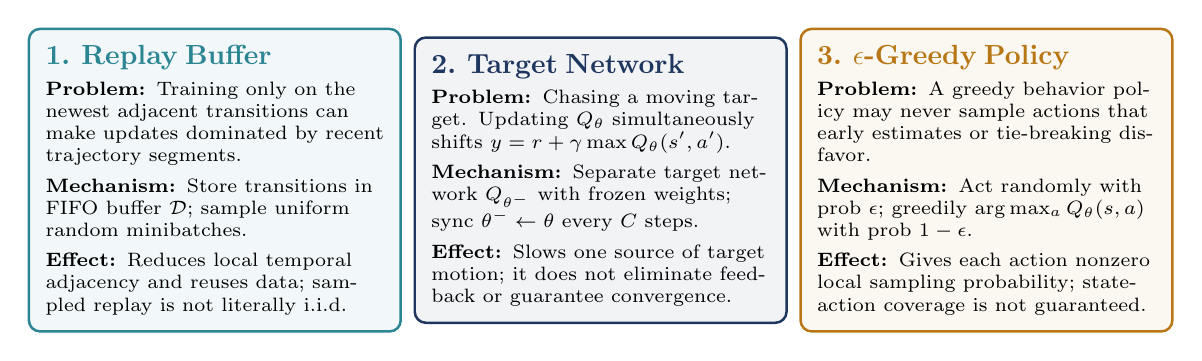
\begin{tikzpicture}[
      pillar/.style={rounded corners=4pt, text width=4.3cm, minimum height=3.5cm, align=left, inner sep=6pt, font=\scriptsize, line width=0.9pt}
    ]
      % Pillar 1: Replay Buffer
      \node[pillar, draw=islteal, fill=islteal!6] (p1) at (2.4, 1.9) {
        {\normalsize\bfseries\color{islteal} 1. Replay Buffer}\\[3pt]
        \textbf{Problem:} Training only on the newest adjacent transitions can make updates dominated by recent trajectory segments.\\[3pt]
        \textbf{Mechanism:} Store transitions in FIFO buffer $\mathcal{D}$; sample uniform random minibatches.\\[3pt]
        \textbf{Effect:} Reduces local temporal adjacency and reuses data; sampled replay is not literally i.i.d.
      };

      % Pillar 2: Target Network
      \node[pillar, draw=islnavy, fill=islnavy!6] (p2) at (7.3, 1.9) {
        {\normalsize\bfseries\color{islnavy} 2. Target Network}\\[3pt]
        \textbf{Problem:} Chasing a moving target. Updating $Q_\theta$ simultaneously shifts $y = r + \gamma \max Q_\theta(s', a')$.\\[3pt]
        \textbf{Mechanism:} Separate target network $Q_{\theta^-}$ with frozen weights; sync $\theta^- \leftarrow \theta$ every $C$ steps.\\[3pt]
        \textbf{Effect:} Slows one source of target motion; it does not eliminate feedback or guarantee convergence.
      };

      % Pillar 3: Epsilon Greedy
      \node[pillar, draw=islgold, fill=islgold!6] (p3) at (12.2, 1.9) {
        {\normalsize\bfseries\color{islgold} 3. $\epsilon$-Greedy Policy}\\[3pt]
        \textbf{Problem:} A greedy behavior policy may never sample actions that early estimates or tie-breaking disfavor.\\[3pt]
        \textbf{Mechanism:} Act randomly with prob $\epsilon$; greedily $\arg\max_a Q_\theta(s, a)$ with prob $1-\epsilon$.\\[3pt]
        \textbf{Effect:} Gives each action nonzero local sampling probability; state-action coverage is not guaranteed.
      };
    \end{tikzpicture}
  \par}
\end{frame}

% ==========================================
% SLIDE 6: Complete DQN Training Loop Diagram
% ==========================================
\begin{frame}{The Complete Deep Q-Network (DQN) System Architecture}
  \sectionlabel{How environment interaction, replay buffer, online network, and target network interact}

  {\centering
    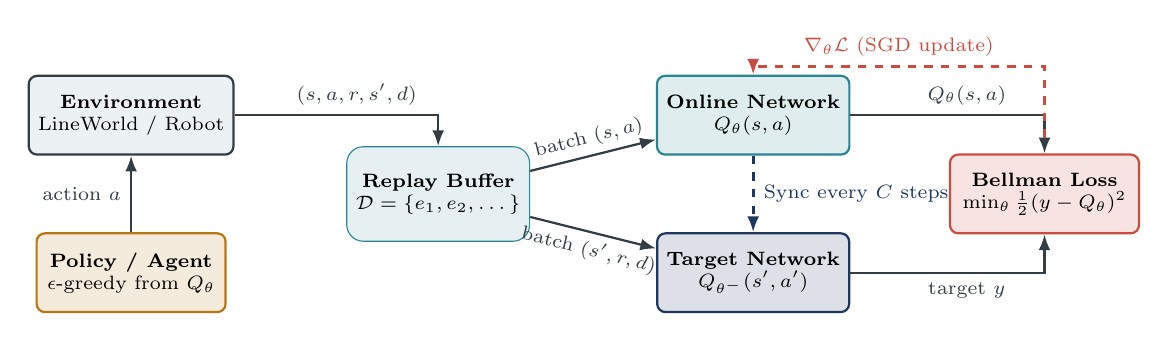
\begin{tikzpicture}[
      box/.style={rectangle, rounded corners=3pt, minimum width=2.4cm, minimum height=1.0cm, align=center, draw=isldark, line width=0.8pt, font=\scriptsize},
      data/.style={rectangle, rounded corners=6pt, draw=islteal, fill=islteal!12, minimum width=2.2cm, minimum height=1.2cm, font=\scriptsize, align=center},
      arr/.style={-{Latex[length=2.0mm]}, thick, color=isldark}
    ]
      % Left Column: Agent & Environment
      \node[box, fill=isllight] (env) at (1.5, 3.1) {\textbf{Environment}\\LineWorld / Robot};
      \node[box, fill=islgold!15, draw=islgold] (policy) at (1.5, 1.1) {\textbf{Policy / Agent}\\$\epsilon$-greedy from $Q_\theta$};

      % Center Column: Replay Buffer
      \node[data] (buffer) at (5.4, 2.1) {\textbf{Replay Buffer}\\$\mathcal{D} = \{e_1, e_2, \dots\}$};

      % Right Column: Networks
      \node[box, fill=islteal!15, draw=islteal] (q_online) at (9.4, 3.1) {\textbf{Online Network}\\$Q_\theta(s, a)$};
      \node[box, fill=islnavy!15, draw=islnavy] (q_target) at (9.4, 1.1) {\textbf{Target Network}\\$Q_{\theta^-}(s', a')$};

      % Far Right: Loss Node
      \node[box, fill=islred!15, draw=islred] (loss) at (13.1, 2.1) {\textbf{Bellman Loss}\\$\min_\theta \tfrac{1}{2}(y - Q_\theta)^2$};

      % Forward Paths
      \draw[arr] (policy) -- (env) node[midway, left]{\scriptsize action $a$};
      \draw[arr] (env) -| (buffer.north) node[pos=0.3, above]{\scriptsize $(s, a, r, s', d)$};
      \draw[arr] (buffer) -- (q_online) node[midway, above=-1pt, sloped]{\scriptsize batch $(s, a)$};
      \draw[arr] (buffer) -- (q_target) node[midway, below=-1pt, sloped]{\scriptsize batch $(s', r, d)$};
      \draw[arr] (q_online) -| (loss.north) node[pos=0.3, above]{\scriptsize $Q_\theta(s,a)$};
      \draw[arr] (q_target) -| (loss.south) node[pos=0.3, below]{\scriptsize target $y$};

      % Feedback & Sync Loops
      \draw[arr, dashed, color=islred, line width=1pt] (loss.north) ++(0, 0.2) -- ++(0, 0.9) -| (q_online.north) node[pos=0.25, above]{\scriptsize $\nabla_\theta \mathcal{L}$ (SGD update)};
      \draw[arr, dashed, color=islnavy, line width=1pt] (q_online.south) -- (q_target.north) node[midway, right]{\scriptsize Sync every $C$ steps};
    \end{tikzpicture}
  \par}
\end{frame}

% ==========================================
% SLIDE 7: Code Lens - Linear Q Checkpoints
% ==========================================
\begin{frame}{Code Lens: From Gradient Update to Evaluation}
  \sectionlabel{Transparent linear function approximation in examples/week-03}

  \begin{columns}[T,onlytextwidth]
    \column{0.48\textwidth}
      {\small\bfseries\color{islteal} Linear Parametric Model}
      \vspace{0.1cm}
      \begin{block}{\footnotesize Parametric Form}
        $Q_\theta(s, a) = w_{0, a} + w_{1, a} \cdot \left(\frac{s}{S_{\max}-1}\right)$
      \end{block}
      \vspace{0.1cm}
      {\footnotesize
      $\bullet$ Feature vector for state $s$: $\phi(s) = [1.0,\, s / 4.0]$.\\[2pt]
      $\bullet$ \textbf{Sparse Parameter Update:} Only weights for the executed action $a$ receive non-zero gradients!\\[2pt]
      $\bullet$ $\nabla_{\theta_a} Q_\theta(s, a) = \phi(s)$.\\[2pt]
      $\bullet$ Weight update: $\theta_a \leftarrow \theta_a + \alpha \cdot \delta \cdot \phi(s)$.
      }

    \column{0.48\textwidth}
      {\small\bfseries\color{islgreen} Empirical Evaluation}
      \vspace{0.1cm}
      \renewcommand{\arraystretch}{1.15}
      \setlength{\tabcolsep}{4pt}
      {\centering
        \footnotesize
        \begin{tabular}{@{}lcc@{}}
          \toprule
          \textbf{Policy} & \textbf{Avg Return} & \textbf{Success Rate} \\
          \midrule
          Random Policy & $+0.52$ & $65\%$ \\
          Always Right (Heuristic) & $+0.97$ & $100\%$ \\
          \textbf{Linear Q-Learner} & $\mathbf{+0.97}$ & $\mathbf{100\%}$ \\
          \bottomrule
        \end{tabular}
      \par}
      \vspace{0.14cm}
      \begin{alertblock}{\footnotesize Diagnostic Discipline}
        Never rely on Bellman loss alone. Low loss can coincide with poor policies if targets or sampled distributions are degenerate. Always evaluate episode returns.
      \end{alertblock}
  \end{columns}
\end{frame}

% ==========================================
% SLIDE 8: Failure Modes & Debugging Guide
% ==========================================
\begin{frame}{Failure Modes in Value Function Approximation}
  \sectionlabel{Common engineering and theoretical pitfalls in DQN implementations}

  {\centering
    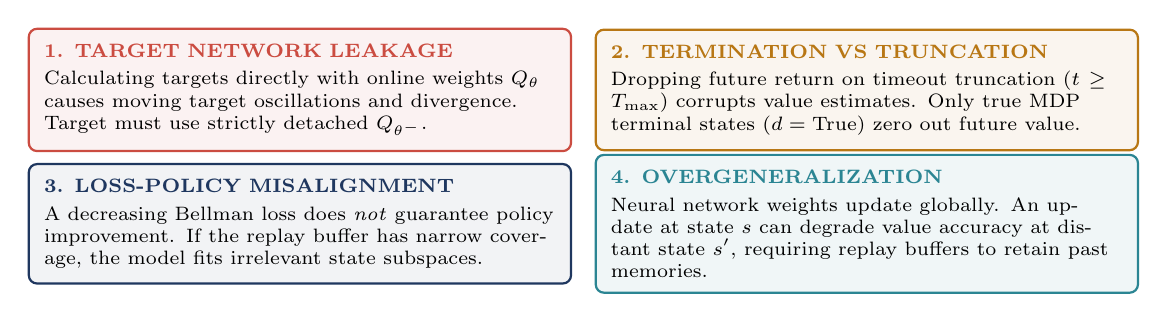
\begin{tikzpicture}[
      card/.style={rounded corners=3pt, text width=6.5cm, minimum height=1.30cm, align=left, inner sep=5.5pt, font=\scriptsize, line width=0.8pt}
    ]
      \node[card, draw=islred, fill=islred!7] at (3.5, 3.1) {
        {\bfseries\color{islred} 1. TARGET NETWORK LEAKAGE}\\[2pt]
        Calculating targets directly with online weights $Q_\theta$ causes moving target oscillations and divergence. Target must use strictly detached $Q_{\theta^-}$.
      };

      \node[card, draw=islgold, fill=islgold!7] at (10.7, 3.1) {
        {\bfseries\color{islgold} 2. TERMINATION VS TRUNCATION}\\[2pt]
        Dropping future return on timeout truncation ($t \ge T_{\max}$) corrupts value estimates. Only true MDP terminal states ($d=\text{True}$) zero out future value.
      };

      \node[card, draw=islnavy, fill=islnavy!6] at (3.5, 1.4) {
        {\bfseries\color{islnavy} 3. LOSS-POLICY MISALIGNMENT}\\[2pt]
        A decreasing Bellman loss does \textit{not} guarantee policy improvement. If the replay buffer has narrow coverage, the model fits irrelevant state subspaces.
      };

      \node[card, draw=islteal, fill=islteal!7] at (10.7, 1.4) {
        {\bfseries\color{islteal} 4. OVERGENERALIZATION}\\[2pt]
        Neural network weights update globally. An update at state $s$ can degrade value accuracy at distant state $s'$, requiring replay buffers to retain past memories.
      };
    \end{tikzpicture}
  \par}
\end{frame}

% ==========================================
% SLIDE 9: Robotics Bridge & Future Outlook
% ==========================================
\begin{frame}{Robotics Bridge: From DQN to Physical Systems}
  \sectionlabel{Why continuous robot control adapts Bellman regression into Actor-Critic methods}

  \begin{columns}[T,onlytextwidth]
    \column{0.48\textwidth}
      {\small\bfseries\color{islnavy} Robotic Observation Spaces}\par\vspace{0.08cm}
      {\footnotesize
      $\bullet$ Joint positions, velocities, torques ($\mathbb{R}^7$).\\[2pt]
      $\bullet$ End-effector 6D poses \& tactile feedback.\\[2pt]
      $\bullet$ Camera RGB-D streams ($224 \times 224 \times 4$).\\[2pt]
      $\bullet$ Language task embeddings (e.g., CLIP / T5).\\[3pt]}
      \begin{block}{\footnotesize High-Dimensional State}
        DQN's core insight (neural value approximation) is mandatory for robot state representation.
      \end{block}

    \column{0.48\textwidth}
      {\small\bfseries\color{islteal} The Action Space Bottleneck}\par\vspace{0.08cm}
      {\footnotesize
      $\bullet$ DQN requires computing $\arg\max_{a \in A} Q(s, a)$.\\[2pt]
      $\bullet$ For continuous torque/velocity actions ($a \in \mathbb{R}^d$), discrete $\max$ optimization is intractable.\\[3pt]
      \textbf{Transition to Actor-Critic (Weeks 5--7):}\\[2pt]
      \quad $\star$ \textbf{Critic:} Evaluates Bellman error $Q_\phi(s, a)$.\\
      \quad $\star$ \textbf{Actor:} Parametric policy $\pi_\theta(s)$ directly outputs continuous actions.}
  \end{columns}
\end{frame}

% ==========================================
% SLIDE 10: Quiz Part 1 - Concepts Check
% ==========================================
\begin{frame}{Week 03 Quiz: Core Concepts \& Mechanisms}
  \sectionlabel{Self-check: verify fundamental understanding of value approximation}

  \begin{center}
    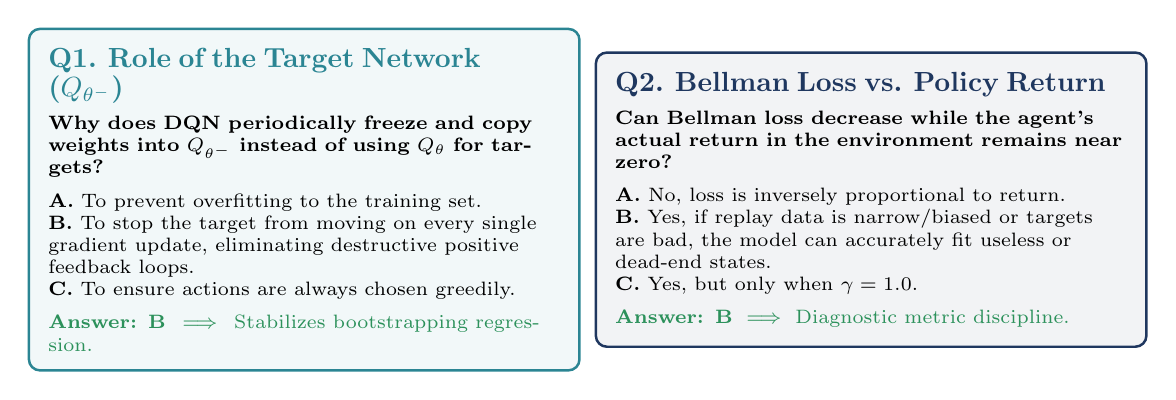
\begin{tikzpicture}[
      qcard/.style={rounded corners=4pt, text width=6.5cm, minimum height=3.3cm, align=left, inner sep=7pt, font=\scriptsize, line width=0.9pt}
    ]
      % Question 1
      \node[qcard, draw=islteal, fill=islteal!6] at (3.5, 1.7) {
        {\bfseries\color{islteal}\normalsize Q1. Role of the Target Network ($Q_{\theta^-}$)}\\[4pt]
        \textbf{Why does DQN periodically freeze and copy weights into $Q_{\theta^-}$ instead of using $Q_\theta$ for targets?}\\[4pt]
        \textbf{A.} To prevent overfitting to the training set.\\
        \textbf{B.} To stop the target from moving on every single gradient update, eliminating destructive positive feedback loops.\\
        \textbf{C.} To ensure actions are always chosen greedily.
        \vskip4pt
        {\color{islgreen}\textbf{Answer: B} $\implies$ Stabilizes bootstrapping regression.}
      };

      % Question 2
      \node[qcard, draw=islnavy, fill=islnavy!6] at (10.7, 1.7) {
        {\bfseries\color{islnavy}\normalsize Q2. Bellman Loss vs. Policy Return}\\[4pt]
        \textbf{Can Bellman loss decrease while the agent's actual return in the environment remains near zero?}\\[4pt]
        \textbf{A.} No, loss is inversely proportional to return.\\
        \textbf{B.} Yes, if replay data is narrow/biased or targets are bad, the model can accurately fit useless or dead-end states.\\
        \textbf{C.} Yes, but only when $\gamma = 1.0$.
        \vskip4pt
        {\color{islgreen}\textbf{Answer: B} $\implies$ Diagnostic metric discipline.}
      };
    \end{tikzpicture}
  \end{center}
\end{frame}

% ==========================================
% SLIDE 11: Quiz Part 2 - Target & Loss Arithmetic
% ==========================================
\begin{frame}{Week 03 Quiz: Target \& TD Error Arithmetic}
  \sectionlabel{Verify hand-computations for terminal vs non-terminal Bellman targets}

  \begin{center}
    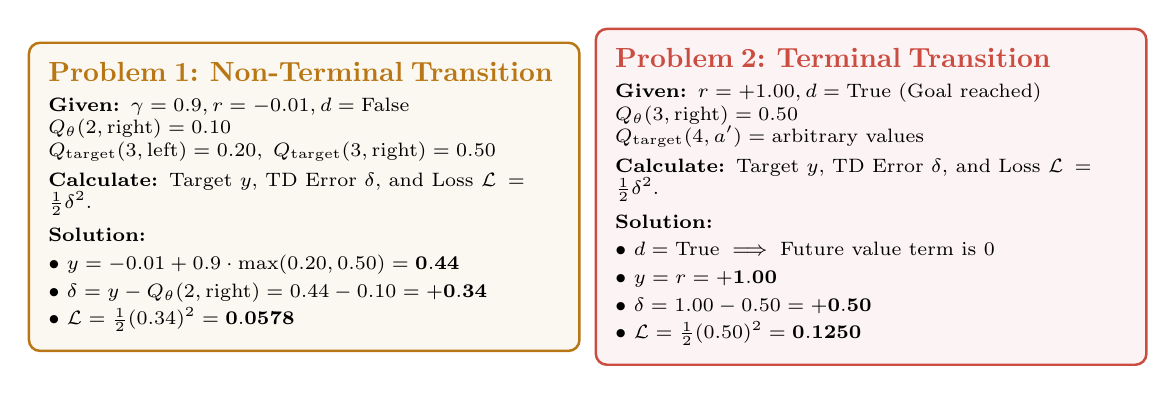
\begin{tikzpicture}[
      qcard/.style={rounded corners=4pt, text width=6.5cm, minimum height=3.3cm, align=left, inner sep=7pt, font=\scriptsize, line width=0.9pt}
    ]
      % Problem 1
      \node[qcard, draw=islgold, fill=islgold!6] at (3.5, 1.7) {
        {\bfseries\color{islgold}\normalsize Problem 1: Non-Terminal Transition}\\[3pt]
        \textbf{Given:} $\gamma=0.9, r=-0.01, d=\text{False}$\\
        $Q_\theta(2, \text{right}) = 0.10$\\
        $Q_{\text{target}}(3, \text{left}) = 0.20, \; Q_{\text{target}}(3, \text{right}) = 0.50$\\[3pt]
        \textbf{Calculate:} Target $y$, TD Error $\delta$, and Loss $\mathcal{L}=\tfrac12\delta^2$.\\[4pt]
        \textbf{Solution:}\\[2pt]
        $\bullet$ $y = -0.01 + 0.9 \cdot \max(0.20, 0.50) = \mathbf{0.44}$\\[2pt]
        $\bullet$ $\delta = y - Q_\theta(2, \text{right}) = 0.44 - 0.10 = \mathbf{+0.34}$\\[2pt]
        $\bullet$ $\mathcal{L} = \tfrac12(0.34)^2 = \mathbf{0.0578}$
      };

      % Problem 2
      \node[qcard, draw=islred, fill=islred!6] at (10.7, 1.7) {
        {\bfseries\color{islred}\normalsize Problem 2: Terminal Transition}\\[3pt]
        \textbf{Given:} $r=+1.00, d=\text{True} \text{ (Goal reached)}$\\
        $Q_\theta(3, \text{right}) = 0.50$\\
        $Q_{\text{target}}(4, a') = \text{arbitrary values}$\\[3pt]
        \textbf{Calculate:} Target $y$, TD Error $\delta$, and Loss $\mathcal{L}=\tfrac12\delta^2$.\\[4pt]
        \textbf{Solution:}\\[2pt]
        $\bullet$ $d=\text{True} \implies \text{Future value term is 0}$\\[2pt]
        $\bullet$ $y = r = \mathbf{+1.00}$\\[2pt]
        $\bullet$ $\delta = 1.00 - 0.50 = \mathbf{+0.50}$\\[2pt]
        $\bullet$ $\mathcal{L} = \tfrac12(0.50)^2 = \mathbf{0.1250}$
      };
    \end{tikzpicture}
  \end{center}
\end{frame}

% ==========================================
% SLIDE 12: Quiz Part 3 - System Design & Diagnostics
% ==========================================
\begin{frame}{Week 03 Quiz: Stabilizers \& Implementation Traps}
  \sectionlabel{Key practical questions every RL practitioner must master}

  \begin{center}
    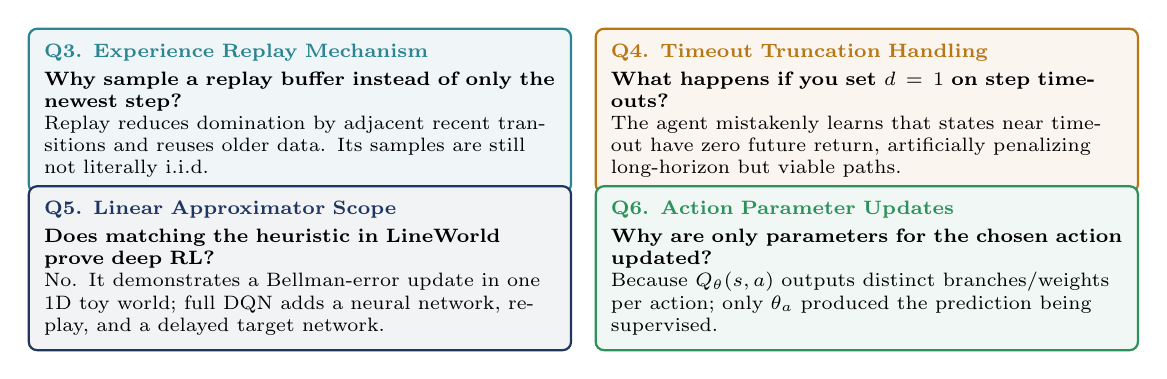
\begin{tikzpicture}[
      card/.style={rounded corners=3pt, text width=6.5cm, minimum height=1.35cm, align=left, inner sep=5.5pt, font=\scriptsize, line width=0.8pt}
    ]
      \node[card, draw=islteal, fill=islteal!7] at (3.5, 3.3) {
        {\bfseries\color{islteal} Q3. Experience Replay Mechanism}\\[2pt]
        \textbf{Why sample a replay buffer instead of only the newest step?}\\
        Replay reduces domination by adjacent recent transitions and reuses older data. Its samples are still not literally i.i.d.
      };

      \node[card, draw=islgold, fill=islgold!7] at (10.7, 3.3) {
        {\bfseries\color{islgold} Q4. Timeout Truncation Handling}\\[2pt]
        \textbf{What happens if you set $d=1$ on step timeouts?}\\
        The agent mistakenly learns that states near timeout have zero future return, artificially penalizing long-horizon but viable paths.
      };

      \node[card, draw=islnavy, fill=islnavy!6] at (3.5, 1.3) {
        {\bfseries\color{islnavy} Q5. Linear Approximator Scope}\\[2pt]
        \textbf{Does matching the heuristic in LineWorld prove deep RL?}\\
        No. It demonstrates a Bellman-error update in one 1D toy world; full DQN adds a neural network, replay, and a delayed target network.
      };

      \node[card, draw=islgreen, fill=islgreen!7] at (10.7, 1.3) {
        {\bfseries\color{islgreen} Q6. Action Parameter Updates}\\[2pt]
        \textbf{Why are only parameters for the chosen action updated?}\\
        Because $Q_\theta(s, a)$ outputs distinct branches/weights per action; only $\theta_a$ produced the prediction being supervised.
      };
    \end{tikzpicture}
  \end{center}
\end{frame}

\end{document}
